\chapter{Circuito de carreras de Fórmula 1}
\label{ch:circuitocarreras}

Una vez explicado el contexto, los objetivos y las herramientas usadas en el proyecto, en este capítulo vamos ver en detalle la construcción de un mundo para Gazebo que se pueda usar en las prácticas de JdeRobot-Academy que emplean coches de carreras, en concreto el circuito de Fórmula 1 de Mónaco.

\section{Prácticas con circuito en JdeRobot-Academy}
\label{sec:circarr_practicas}

Las prácticas del entorno JdeRobot-Academy están diseñadas de forma que tanto el mundo como el robot están correctamente montados y configurados, y la aplicación que controla al robot está parcialmente completa. El alumno no necesita realizar modificaciones al mundo simulado o al robot, pero debe completar el código de la aplicación para realizar las tareas propuestas en la práctica. En la figura \ref{fig:graficof1} podemos ver la relación entre los componentes software de estas prácticas, así como el espacio destinado al trabajo del alumno. Marcado con una flecha roja esta Gazebo, para señalar las partes modificadas con este Trabajo Fin de Grado. No cambiamos nada del coche ni de la aplicación docente, sí cambiamos el mundo de Gazebo para lograr que la misma práctica se situe en otro escenario.

\begin{figure}[h]
	\centering
	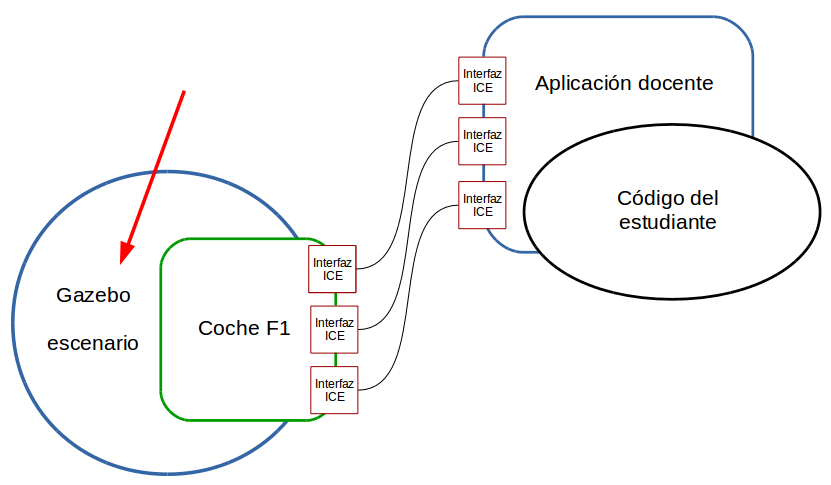
\includegraphics[width=0.8\textwidth]{graficof1.png}
	\caption{Esquema de los componentes de las prácticas con Fórmula 1.} \label{fig:graficof1}
\end{figure}

Actualmente el entorno JdeRobot-Academy presenta dos prácticas basadas en circuitos de Fórmula 1:
\begin{itemize}
	\item Práctica de navegación local autónoma: En esta práctica el Fórmula 1 dispone de unos sensores que le permiten detectar obstáculos. En la figura \ref{fig:vff} podemos apreciar el funcionamiento del sensor comparando la información que recibe con la vista real de la simulación. En esta práctica el alumno ha de rellenar el código con elementos de percepción, que le permitan identificar los obstáculos, y con algoritmos de navegación local como el VFF (visual force field), logrando dar vueltas al circuito esquivando los obstáculo presentes.
	
	\item Práctica de sigue-línea: En esta práctica el Fórmula 1 dispone de una cámara con la que capta imágenes del circuito. En este caso el circuito dispone de una línea roja en el suelo, y el coche ha de seguir esa línea para completar las vueltas. En esta práctica el alumno ha de programar el código con algoritmos de procesamiento de imagen, como filtros de color o de formas, y con elementos de control como controladores PID para que el robot siga la línea.
\end{itemize}
	
\begin{figure}[h]
	\centering
	\subfigure[Vista del simulador.]{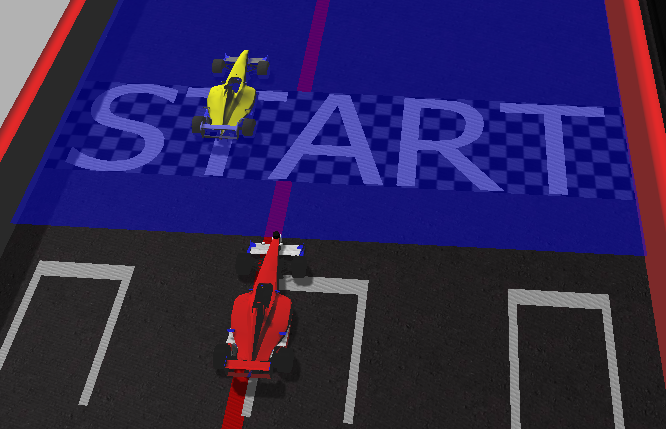
\includegraphics[width=0.47\textwidth]{vff-gazebo.png}}
	\subfigure[vista del sensor.]{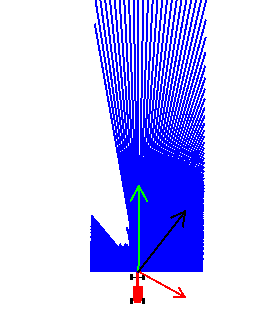
\includegraphics[width=0.25\textwidth]{vff-gui.png}}
	\caption[Vistas de la práctica de navegación local del F1.]{Vistas de la realización de la práctica, tanto lo que muestra Gazebo (a) como una representación de lo que recibe el sensor (b).} \label{fig:vff}
\end{figure}

Nuestro objetivo es reconstruir el circuito de Mónaco de forma que se pueda utilizar en ambas prácticas, creando para ello mundos de Gazebo que se acoplen al esquema de funcionamiento de estas prácticas, como muestra la flecha de la figura \ref{fig:graficof1}.

\section{Manejo de Blender}
\label{sec:circarr_manejodeblender}

En esta sección vamos a explicar cómo se utiliza este potente programa de creación, renderizado y animación de gráficos tridimensionales. El uso de este tipo de programas es, a priori, de los más difíciles, ya que trabajar sobre un mundo tridimensional en una pantalla de ordenador, desplazando un ratón sobre una mesa en dos dimensiones, exige un esfuerzo de abstracción considerable.

Es por ello que en los primeros pasos de esta sección nos dedicaremos a presentar la interfaz del programa y exponer la inmensa cantidad de opciones y herramientas de que dispone, centrándonos en aquellas que han resultado relevantes para la consecución de los objetivos marcados.


\subsection{Interfaz}
\label{subsec:circarr_interfaz}

Como se verá, la interfaz de Blender no sigue el patrón típico de los programas a los que estamos habituados, como editores de texto y hojas de cálculo o entornos de desarrollo de software, por lo que resulta fácil desorientarse al principio.

La interfaz de usuario de Blender está compuesta por 4 ventanas por defecto, como se pueden diferenciar en la figura \ref{fig:interfazblender01}. Cada ventana tiene una cabecera con las herramientas adecuadas para trabajar sobre
dicha ventana y, a su vez, cada herramienta está dotada de sus correspondientes pestañas para una completa edición. Esta disposición facilita y agiliza el uso apropiado del programa. A su vez, cada cabecera de cada ventana tiene el botón Tipo de Editor, mediante el cual se puede cambiar el tipo de ventana que se muestra, por lo que se puede personalizar el aspecto para agilizar el trabajo.

\begin{figure}[ht]
	\centering
	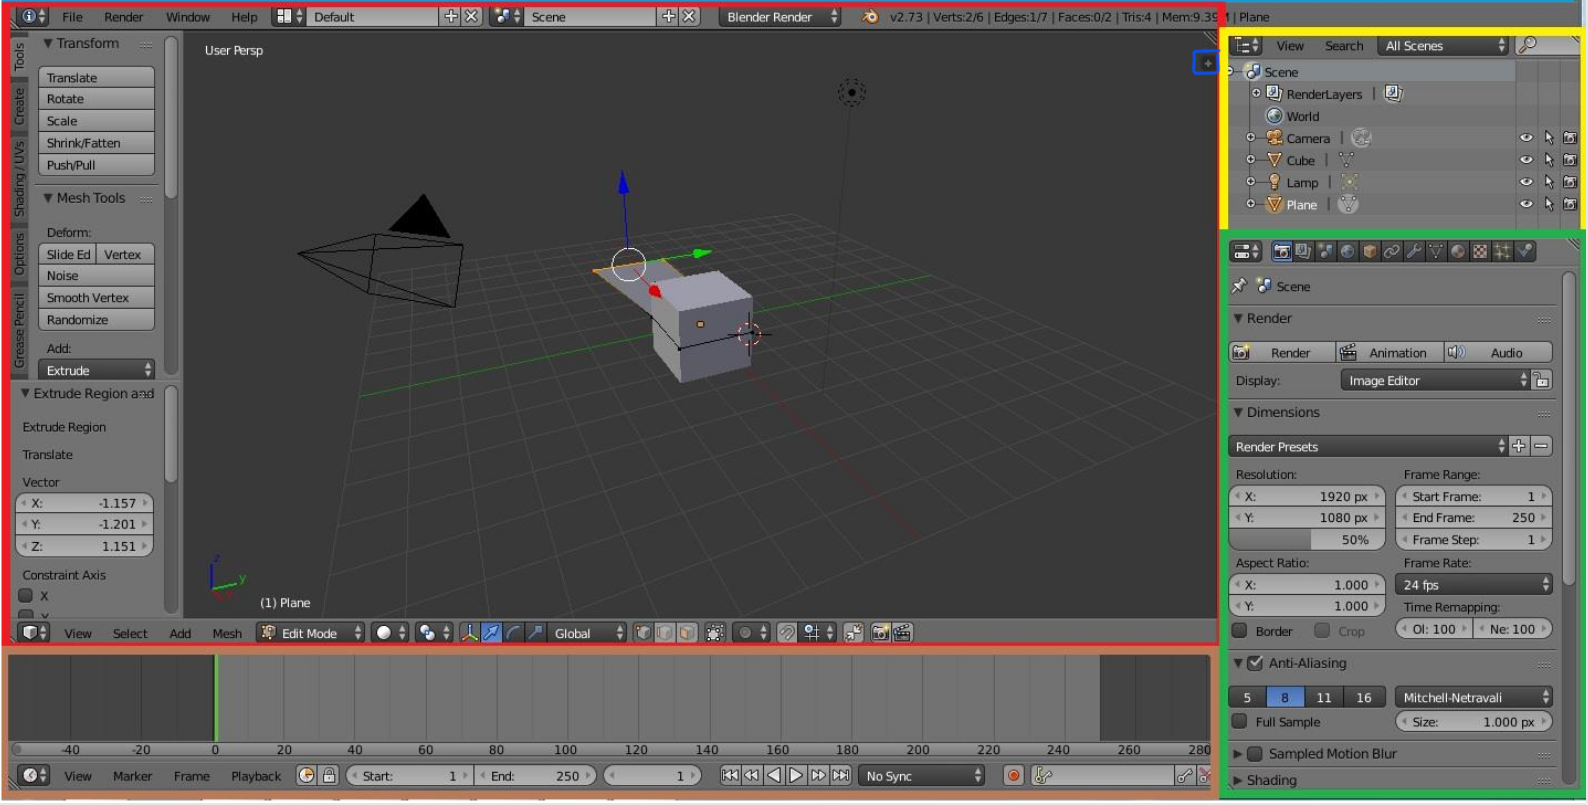
\includegraphics[width=0.9\textwidth]{InterfazBlender01.png}
	\caption{Interfaz de Blender.} \label{fig:interfazblender01}
\end{figure}


En primer lugar tenemos la ventana de Vista 3D, bordeada en color Rojo. En esta ventana se visualiza todo el trabajo y los cambios que se realizan con el programa. En esta ventana podemos observar los siguientes objetos y menús:

\begin{itemize}
	\item Manipuladores de Transformaciones en 3D (\textit{Figura \ref{fig:interfazblender03}}): Muestra de manera visual información de las transformaciones a realizar. Cada objeto puede ser transformado de tres maneras: traslación (G), rotación (R) y escalado (S). Utilizando la combinación Ctrl+Space,	o bien haciendo clic en el icono del sistema de coordenadas, se puede mostrar y ocultar el manipulador. 
	\begin{figure}[h]
		\centering
		
\includegraphics[width=0.30\textwidth]{InterfazBlender03.png}
		\caption{Detalle de Manipuladores de transformaciones en 3D.} \label{fig:interfazblender03}
	\end{figure}
	
	
	\item Cursor 3D (\textit{Figura \ref{fig:interfazblender04}}): El cursor 3D es una herramienta muy útil y se utiliza para una variedad de cosas como representar el lugar donde se añadirán nuevos objetos o representar el punto de pivote para una rotación. Sin embargo, es muy engorroso a la hora de trabajar ya que es muy fácil moverlo accidentalmente y al necesitar usarlo se pierde bastante tiempo reubicándolo.
	\begin{figure}[h]
		\centering
		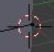
\includegraphics[width=0.12\textwidth]{InterfazBlender04.png}
		\caption{Detalle del cursor de Blender.} \label{fig:interfazblender04}
	\end{figure}

	\item Cubo: Al iniciar Blender, por defecto, aparece un cubo situado en el centro de la ventana 3D. Es uno de los elementos básicos que se pueden insertar y la mayoría de las veces basta este simple cubo para comenzar a trabajar.
	
	\item Luz (de tipo lámpara): Al iniciar Blender, por defecto, también aparecerá una Luz de tipo lámpara que estará en algún sitio cerca del centro de la escena. Es posible crear otras fuentes de luz, como un sol en el cenit de la escena o una luz direccional que ilumine todos los objetos. En cualquier caso, aunque en los diferentes modos de edición no sea necesario, a la hora de renderizar la escena para visualizar el resultado del trabajo es necesaria alguna fuente de luz, si no, aparecerá una escena llena de siluetas.
	
	\item Cámara: Al iniciar Blender, por defecto, aparecerá una cámara que estará en algún sitio por el centro de la ventana 3D y, probablemente, enfocando al cubo. En la figura \ref{fig:interfazblender01} es esa especie de pirámide de vértices negros a la izquierda del cubo. A la hora de renderizar es necesaria una cámara.
	
	\item Objeto seleccionado actualmente: Este campo, situado en la parte inferior izquierda de la escena, al lado del eje de coordenadas, muestra el  nombre del objeto seleccionado actualmente.
	
	\item Modo Edición: Este botón, en forma de desplegable, se encuentra a la izquierda de los botones de manipuladores de transformaciones 3D. Da acceso a un modo de edición para manipular la geometría del objeto. Al activarse aparecen disponibles tres botones de opciones, justo a la derecha de los botones de manipuladores de transformaciones 3D. Nos permiten cambiar entre la selección y edificación de los vértices, de las aristas y de las caras del objeto. La posibilidad de cambiar entre estas opciones de selección es especialmente útil a la hora de dar forma a los objetos que componen el circuito.
	
	\item Vista de la escena: Este botón, en forma de desplegable, se encuentra a la derecha del botón de Modo Edición. Da acceso a un desplegable que permite elegir la vista de la escena 3D entre las posibles, como sólida, texturas, materiales, ”wireframe”, renderizada, etc. Nos permite ver los objetos de la escena con sólo las texturas, sólo los vértices, ya renderizado, etc, para poder trabajar más cómodo en según que condiciones y ver los resultados de aplicar texturas o del renderizado final.
	
\end{itemize}

Para realizar con comodidad el trabajo sobre cualquier tipo de elemento existen diferentes vistas disponibles, cada una con un atajo de teclado propio, en concreto del teclado numérico. De esta forma para el “1” el programa proporciona una vista frontal de la escena; con el número “3” se obtiene una vista derecha; etc. Una de las más cómodas para realizar el trabajo es la que le corresponde al número “7” ya que se trata de una vista cenital, que una vez superpuesto el plano del circuito facilitan la tarea de trazar el recorrido. Por último, con la tecla “5” podemos cambiar la vista de Perspectiva a Ortográfica. La vista Perspectiva es la más similar a la realidad, dando profundidad a la escena y sensación de lejanía y proximidad de los objetos. La vista Ortográfica es más artificial, pues es como una proyección de la anterior, pero es útil en determinadas situaciones para no alterar las proporciones o manejar con fluidez objetos que quedarían tapados de otra forma.

Esta ventana posee un botón de propiedades propio marcado en color Azul en la parte superior derecha, el cual despliega la ventana de propiedades (\textit{Figura \ref{fig:interfazblender02}}). Esta ventana muestra las propiedades del objeto seleccionado y resulta muy útil a la hora de añadir nuevos bloques o realizar modificaciones de los ya existentes, pudiendo modificar la localización, rotación, escala, etc.

\begin{figure}[h]
	\centering
	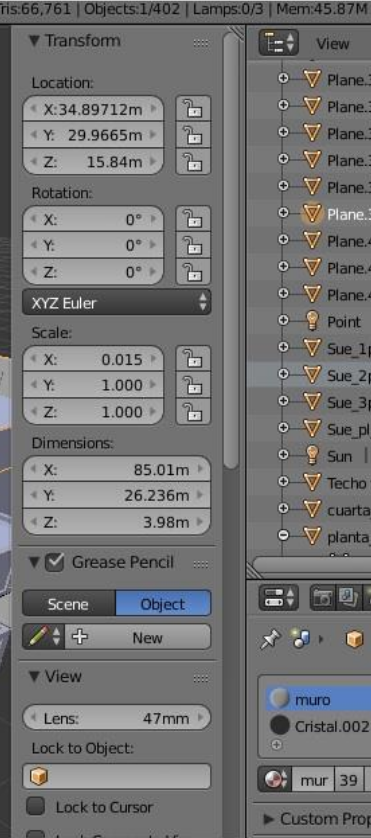
\includegraphics[width=0.4\textwidth]{InterfazBlender02.png}
	\caption{Ventana de propiedades.} \label{fig:interfazblender02}
\end{figure}

Debajo de la ventana de vista 3D, bordeada en marrón, se encuentra por defecto la ventana de Línea Temporal. Aquí se reflejan cronológicamente los bloques u objetos que se han añadido o modificado y es muy utilizada al trabajar con animaciones. En nuestro caso la hemos sustituido por otra que se adapta mejor a nuestras necesidades.

A continuación, bordeada en amarillo, se puede identificar la ventana de Objetos y Jerarquías, donde se pueden ver todos los datos que se utilizan en el trabajo. De esta forma se pueden controlar los diferentes bloques que se utilicen, las luces que se añaden a la escena, cámaras y toda clase de elementos disponibles en la escena. En esta ventana se pueden seleccionar directamente los elementos que se deseen independientemente, y realizar acciones sobre ellos como restringir o habilitar la visualización, selección o renderización de dicho elemento. Esto supone una gran ayuda cuando se superponen diferentes elementos en la ventana.

Debajo de ésta, marcada en color verde, se encuentra la ventana de Propiedades, en la cual se pueden editar las propiedades de los bloques, objetos, materiales, texturas etc. que se utilizan en el trabajo. Esto se consigue mediante los llamados botones de contexto, los cuales muestran un grupo de paneles con opciones diferentes para cada botón. Gracias a esta disposición se esconden multitud de herramientas muy usadas en un espacio reducido y cómodo. Algunas de las tareas que permiten llevar a cabo son: asignar el material o la textura deseada a los elementos creados o modificaciones para replicar, deformar, dividir o desdoblar elementos entre muchas otras opciones

\section{Creación de un circuito plano}
\label{sec:circarr_circuitoplano}

Una vez presentadas las opciones básicas de Blender y cómo desenvolverse entre ellas con un mínimo de soltura pasaremos a desarrollar el proceso de creación del circuito de Mónaco. En este proyecto comenzamos creando el trazado del circuito  sin elevaciones, para coger soltura en el manejo del programa y explorar las diferentes opciones antes de realizar tareas más complejas. 

Vamos a replicar en Blender los diferentes tramos y elementos del circuito como distintos objetos con textura, materiales, etc. Los juntaremos con un objeto plano compuesto que también tiene el mar para conseguir recrear el trazado y sus alrededores.

\begin{figure}[ht]
	\centering
	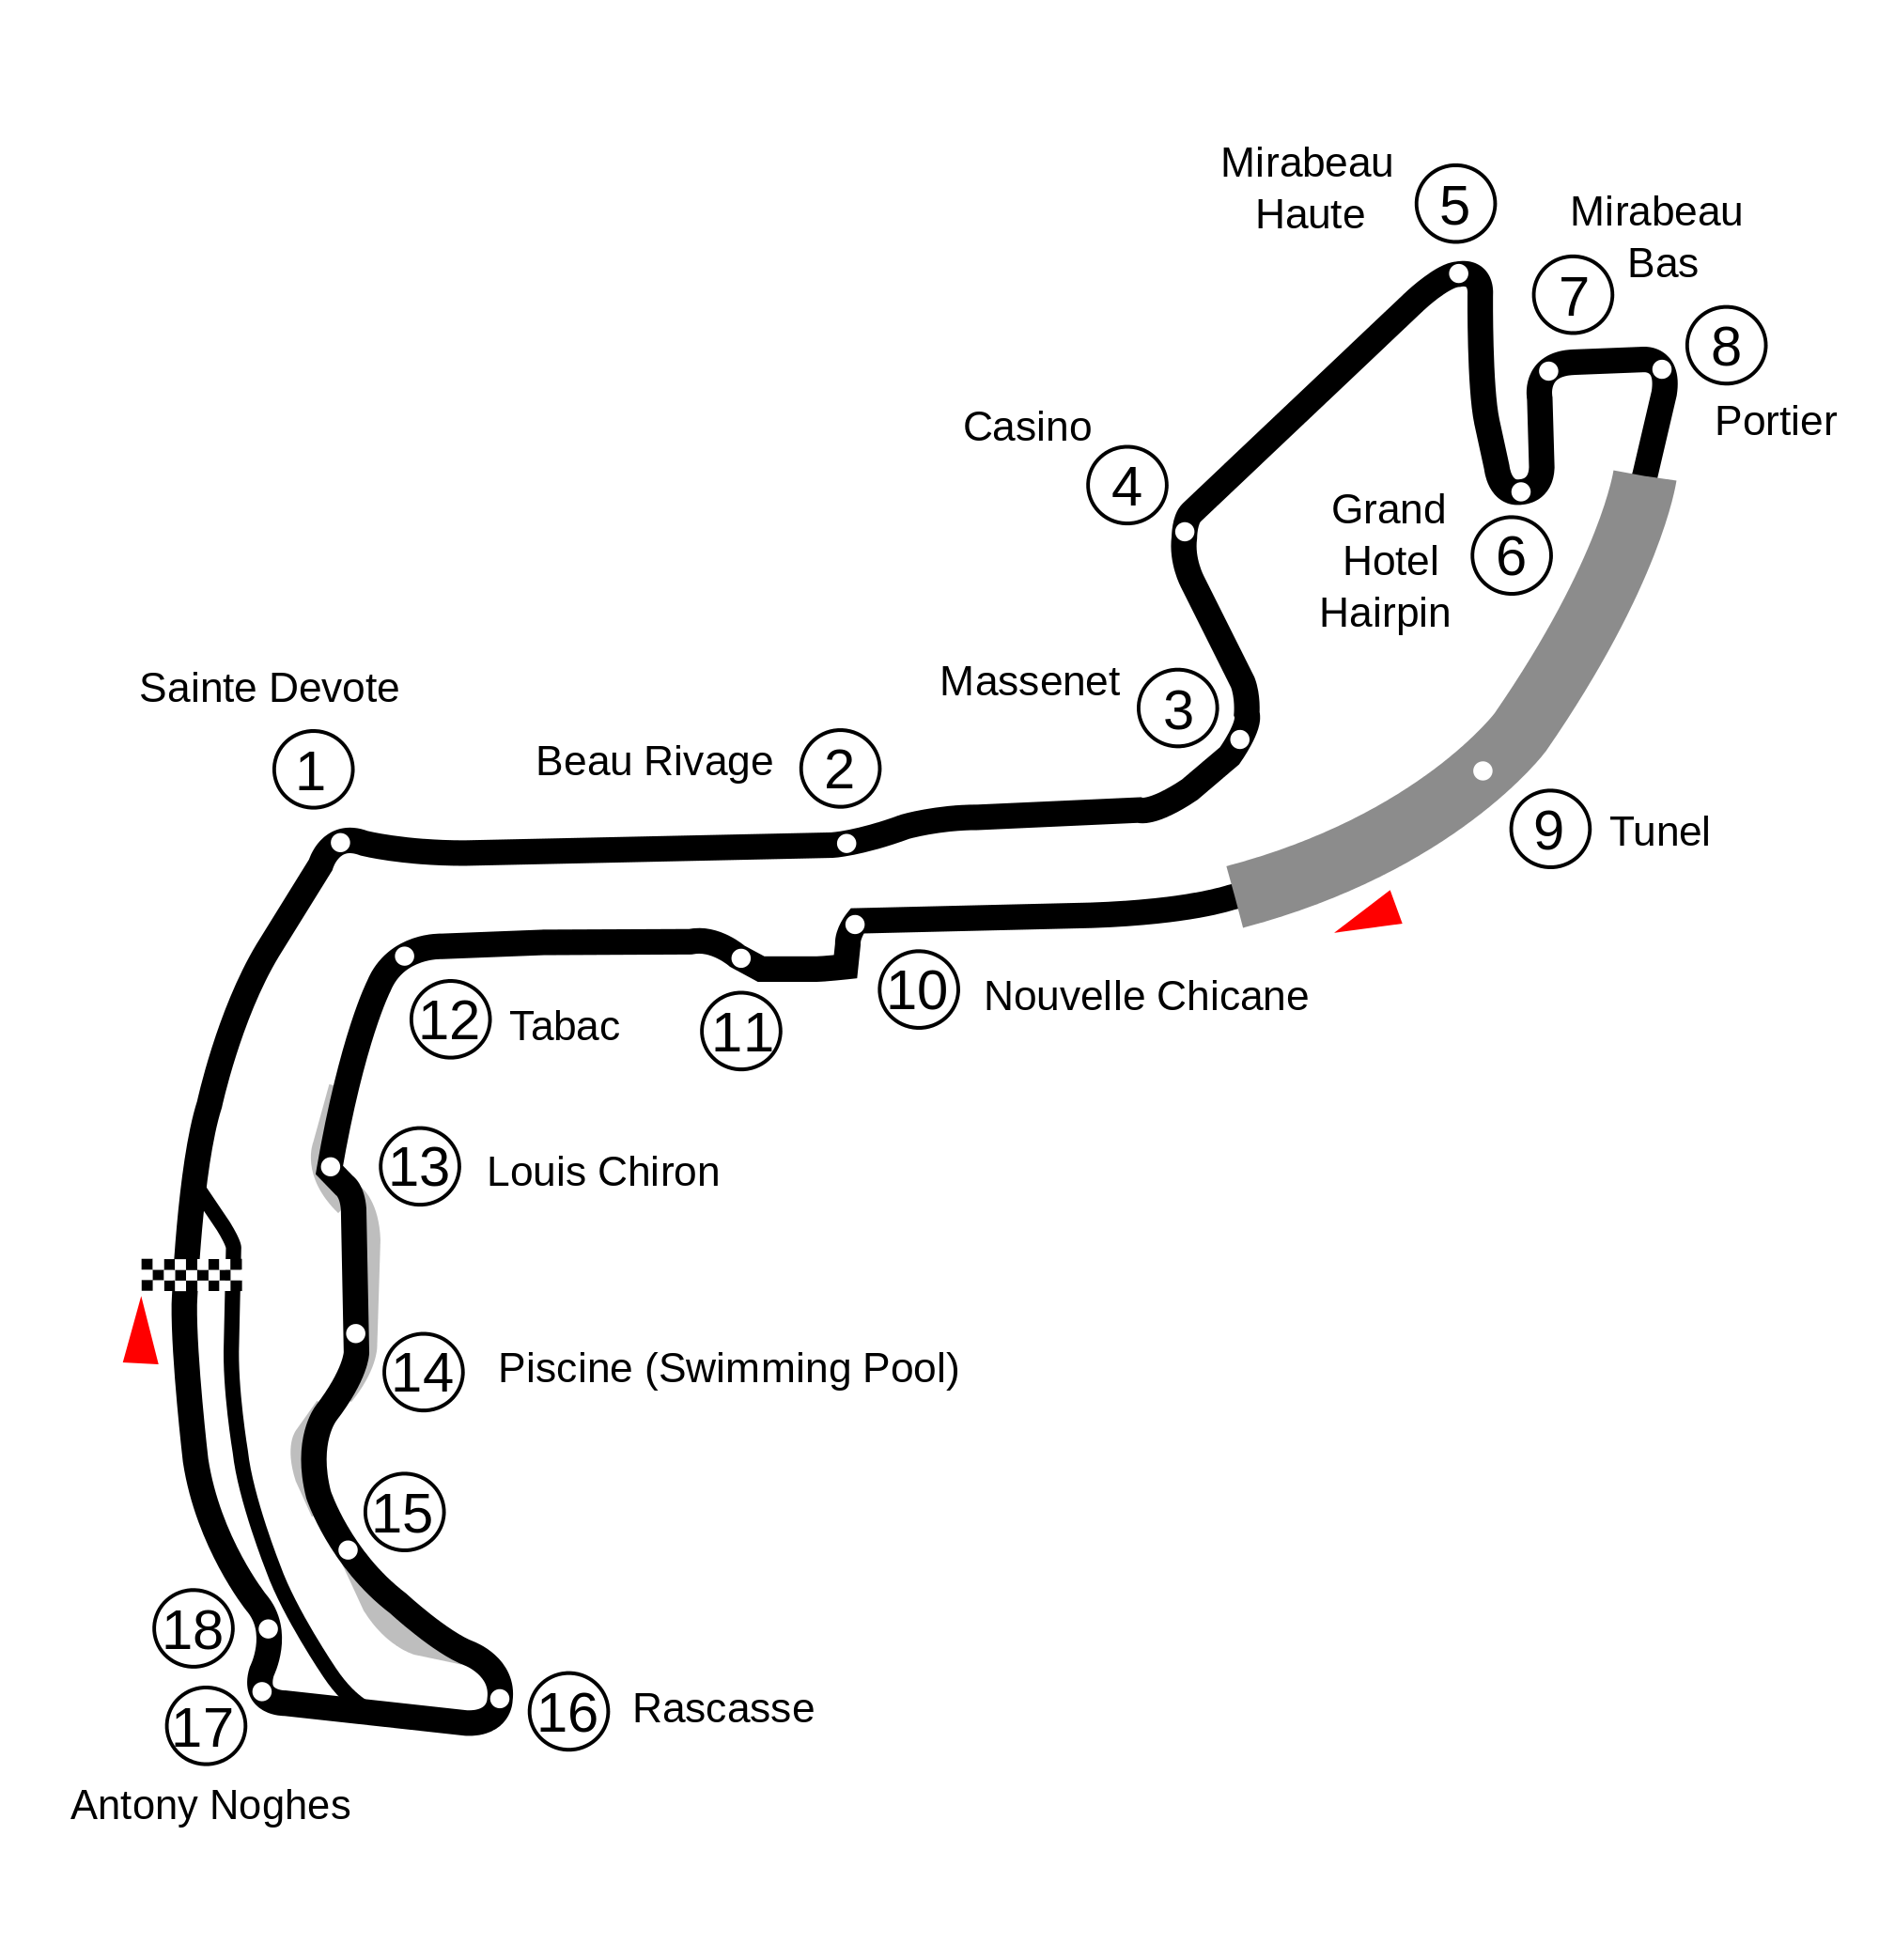
\includegraphics[width=0.5\textwidth]{CircuitoMonaco.png}
	\caption{Trazado del circuito de Mónaco usado como plantilla.} \label{fig:circuitomonaco}
\end{figure}

Comenzamos eliminando el cubo que aparece por defecto, desplegando la ventana de propiedades del menú principal y buscando el apartado de “Background Images”. Activamos la casilla y buscamos la imagen que deseamos poner de fondo, en este caso la imagen de la figura  \ref{fig:circuitomonaco}. Es el trazado real del circuito, visto desde arriba. Lo usaremos como plantilla creando curvas y tramos de carretera en Blender que se solapen con estas. Al hacer click en el botón “Add Image” podremos seleccionar la imagen que queremos ver de fondo, así como el eje en el que la queramos ver. Esta herramienta es especialmente útil ya que  nos permite ver una superposición de la imagen del trazado al usar la vista cenital, que corresponde con la tecla “7” del teclado numérico, pero en cualquier otro ángulo no se verá, con lo que facilita enormemente la tarea de escalado y modelado del circuito.

A continuación añadimos una curva “Bezier” (\textit{Figura \ref{fig:interfazblender05}}), hacemos esto desde el menú superior en \textit{Add}, \textit{Curve}, \textit{Bezier}. Esto creará un nuevo objeto, que podemos renombrar en la ventana de Objetos para facilitar el acceso y la selección posteriormente, cuando tengamos mas objetos en la escena. Este tipo de curvas, como se puede apreciar en la figura \ref{fig:interfazblender05}, son unas curvas com muchos elementos que nos permiten moldearlas a nuestro gusto. En cada extremo del tramo se componen de una recta con tres puntos. el central que establece el inicio del trazo de la curva, y los otros dos que establecen el giro de la curva y lo pronunciado que és. Cuanto más cerca estén del punto central más cerrado será el ángulo de giro, y cuanto más alejados más suave la curva descrita.

\begin{figure}[h]
	\centering
	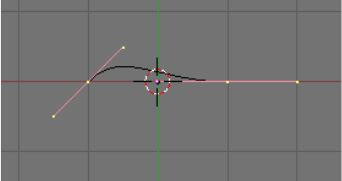
\includegraphics[width=0.5\textwidth]{InterfazBlender05.png}
	\caption{Detalle de curva Bezier.} \label{fig:interfazblender05}
\end{figure}

Al hacer click con el botón izquierdo del ratón mientras mantenemos la tecla Control pulsada añadimos un nuevo punto a la curva ya existente. De esta forma podemos ir añadiendo puntos y deformando la curva hasta que se superponga con la imagen del trazado. Así logramos una curva cerrada correspondiente al trazado sobre la cual situar los elementos que compondrán la carretera, como podemos apreciar en la Figura \ref{fig:monacotrazado} (\textit{La línea naranja es la curva Bezier que será el trazado}).

A continuación añadimos un plano haciendo \textit{Add}, \textit{Mesh}, \textit{Plane}, lo cual generará un cuadrado plano en el centro de la escena A continuación seleccionamos una arista y la extruimos (\textit{estiramos}) dos veces, una más corta y una más larga. hacemos lo mismo con la arista opuesta del cuadrado. Es importante realizar este paso ayudándonos de las flechas de colores (\textit{verde, rojo y azul}) que aparecen al seleccionar un objeto para mantener el conjunto en el mismo plano. Una vez realizado, extruimos los dos rectángulos más pequeños hacia arriba, consiguiendo crear la carretera, las vallas y una acera para el circuito, aunque de momento sólo aparecen en gris.

\begin{figure}[ht]
	\centering
	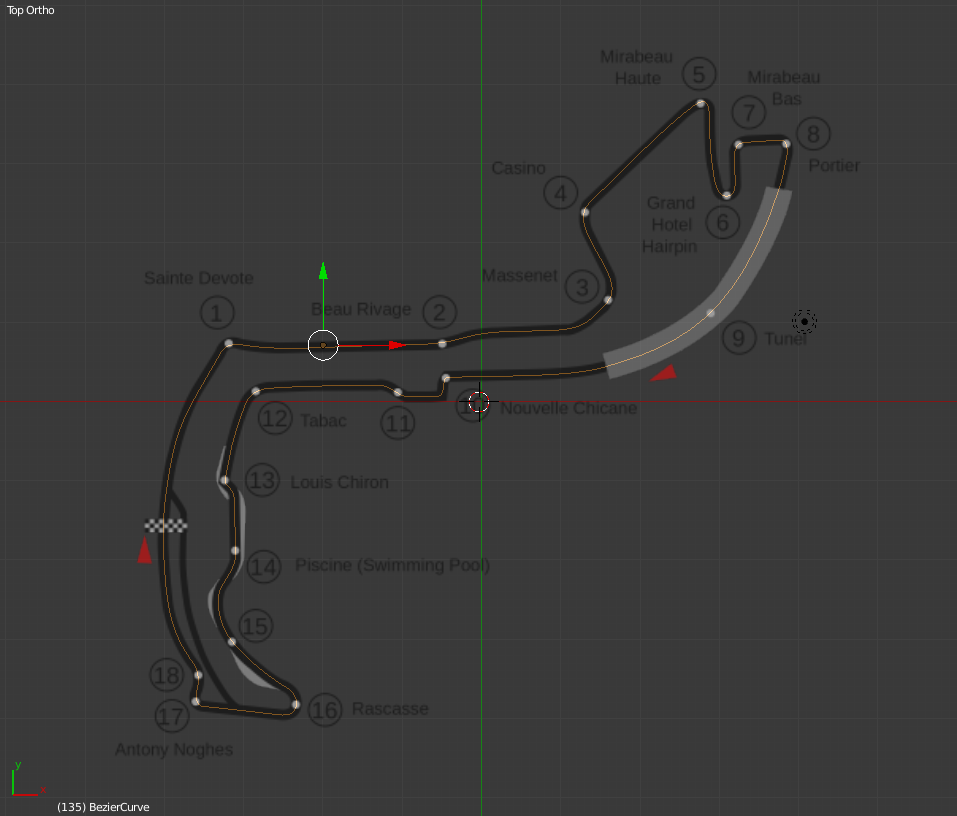
\includegraphics[width=0.85\textwidth]{MonacoTrazado.png}
	\caption{Trazado del circuito de Mónaco superpuesto a la plantilla.} \label{fig:monacotrazado}
\end{figure}

Para ayudarnos en la labor de texturizar objetos, editamos el tipo de ventana que es la de la parte inferior, el gráfico temporal, y lo sustituimos por un Editor de Imagen/UV, el cual posee herramientas avanzadas de manejo de imágenes para texturizado de superficies. De esta manera vamos cara por cara de nuestro objeto seleccionándola en la vista 3D, añadiendo una textura\footnote{Las imágenes usadas como texturas y materiales en este proyecto han sido obtenidas de manera gratuita de la página textures.com\cite{texturescom}} en el Editor UV, y observando los resultados en la vista 3D cambiando el modo de visualización a texturizado. La ventana del Editor de imagen nos sirve para redimensionar las texturas, girarlas, pintar encima de ellas, establecer qué zonas aparecen en la superficie seleccionada, y multitud de herramientas que hacen mucho más sencilla la edición de texturas. Una vez finalizado el paso de texturizar las caras del objeto obtenemos el segmento de la figura \ref{fig:monacosegmento}.

\begin{figure}[h]
	\centering
	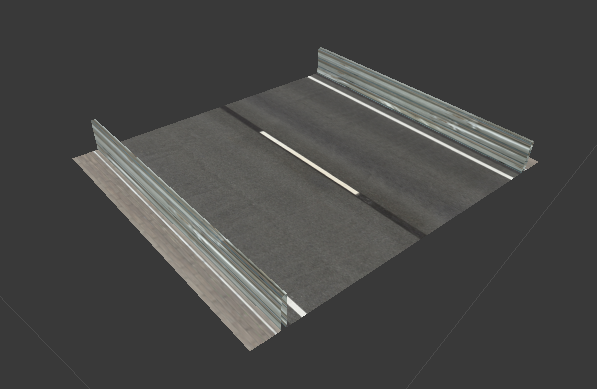
\includegraphics[width=0.5\textwidth]{MonacoSegmento.png}
	\caption{Segmento del circuito.} \label{fig:monacosegmento}
\end{figure}

Es muy importante crear un material para cada textura y asignarlo a las caras correspondientes, de otra manera no se aplicará la textura al renderizar y será como haber trabajado en vano. Esto se consigue mediante la ventana de propiedades y haciendo click en la pestaña de materiales. Es necesario crear un material nuevo, añadir como fuente la misma imagen que se ha usado como textura anteriormente, renombrar para no confundirlos más adelante, y asignarlo a la superficie correspondiente. Además, en la pestaña texturas, debemos repetir los pasos para crear la textura de la misma forma que el material. Necesitaremos además asignar cada textura al material correspondiente y cambiar el tipo de mapping a UV. Es una tarea laboriosa pero muy importante, ya que de no realizarse correctamente las texturas podrían no aplicarse y el objeto aparecería gris plano.

\begin{figure}[hb]
	\centering
	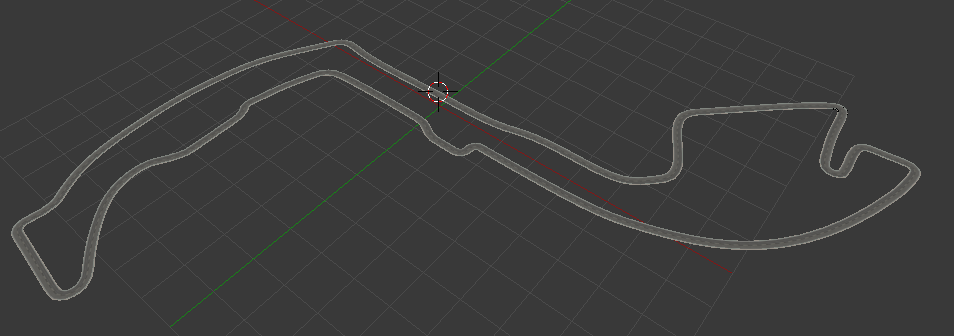
\includegraphics[width=1\textwidth]{MonacoTrazado1.png}
	\caption{Circuito (sólo el trazado).} \label{fig:monacotrazado1}
\end{figure}

Una vez realizados todos estos pasos seleccionamos el segmento del trazado creado y vamos a la ventana de propiedades y hacemos click en la pestaña de modificadores. Añadimos un nuevo modificador, un Array. Con esto conseguimos crear multitud de objetos iguales conectados entre sí, como si de un circuito de \textit{Scalextric} se tratase. Despues añadimos otro modificador, una curva en este caso, y elegimos como elemento modificante la curva Bezier que hemos creado anteriormente. De esta manera, jugando con el número de copias que realiza el array, conseguimos que el segmento creado se repita y deforme siguiendo el trazado de la curva, adquiriendo la forma del circuito deseado. Este método requiere de muchos retoques manuales, ya que en los vértices de las curvas cerradas el programa no puede calcular bien y solapa y deforma de manera incorrecta los vértices del segmento. Una vez realizados todos los retoques, así como la unión del primer y último segmento, obtenemos el objeto de la figura \ref{fig:monacotrazado1}.

Una vez obtenido el primer trazado completo necesitamos añadir un plano que servirá de fondo para el circuito. Para ello añadimos un nuevo objeto plano a la escena, lo aumentamos de tamaño hasta que se pueda situar el circuito en su interior y lo subdividimos en cuadrículas. Esto lo hacemos así para poder asignar texturas a cada cuadrícula independientemente y simular de manera más realista que este circuito se sitúa en un puerto, estando a la orilla del mar casi la mitad de su recorrido. Una vez realizada la división deformamos algunos vértices escondiéndolos debajo del trazado, necesitando así menos divisiones y aligerando la carga de procesamiento para la simulación del circuito. Una vez asignadas todas las texturas, repitiendo los pasos descritos para texturizar el segmento del circuito, obtenemos el circuito de Mónaco (\textit{Figura \ref{fig:monacoplano1}}), el cual podemos ver en detalle en la Figura \ref{fig:monacoplanovistas}.

\begin{figure}[t]
	\centering
	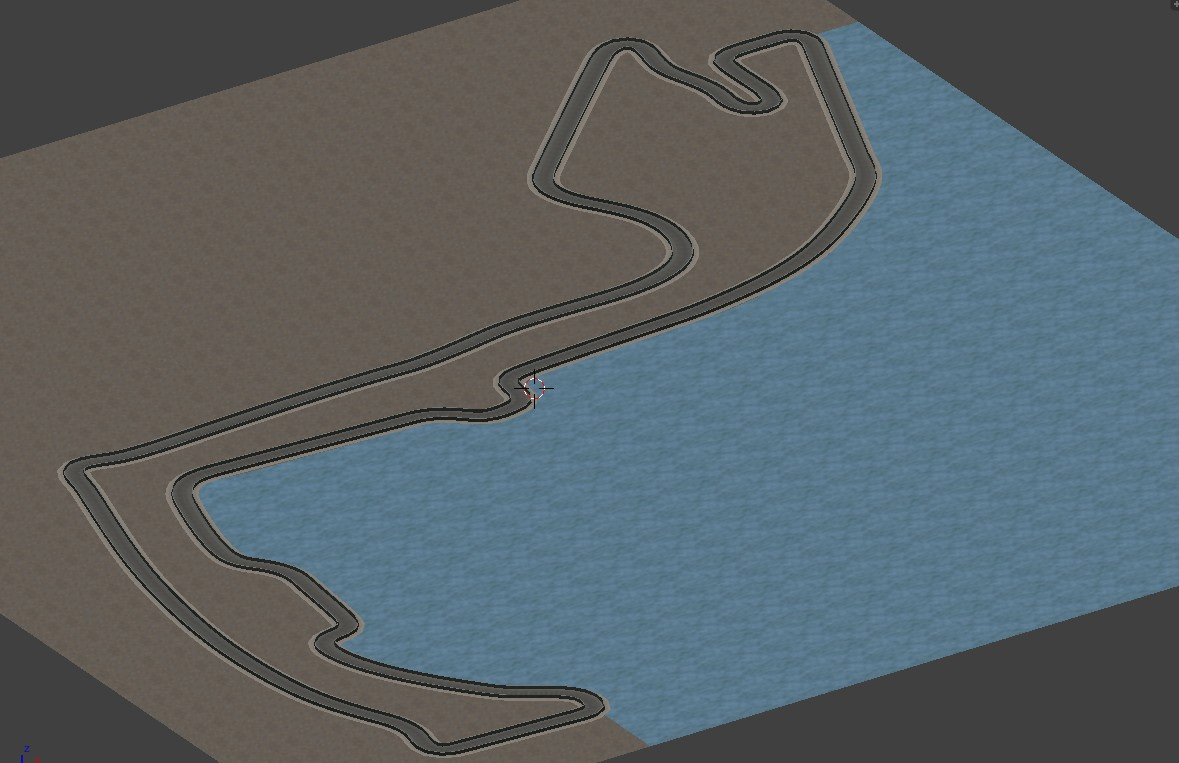
\includegraphics[width=0.7\textwidth]{MonacoPlano1.jpg}
	\caption{Circuito plano.} \label{fig:monacoplano1}
\end{figure}

\begin{figure}
	\centering
	\subfigure{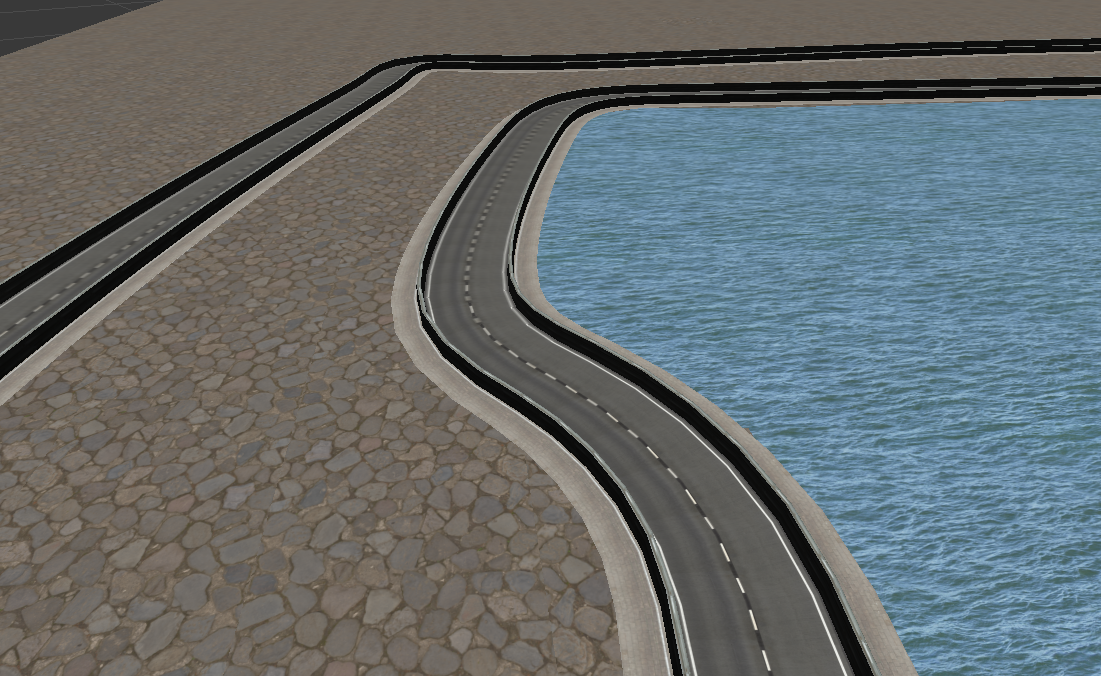
\includegraphics[width=0.47\textwidth]{MonacoPlano2.png}}\hspace{0.02\textwidth}	
	\subfigure{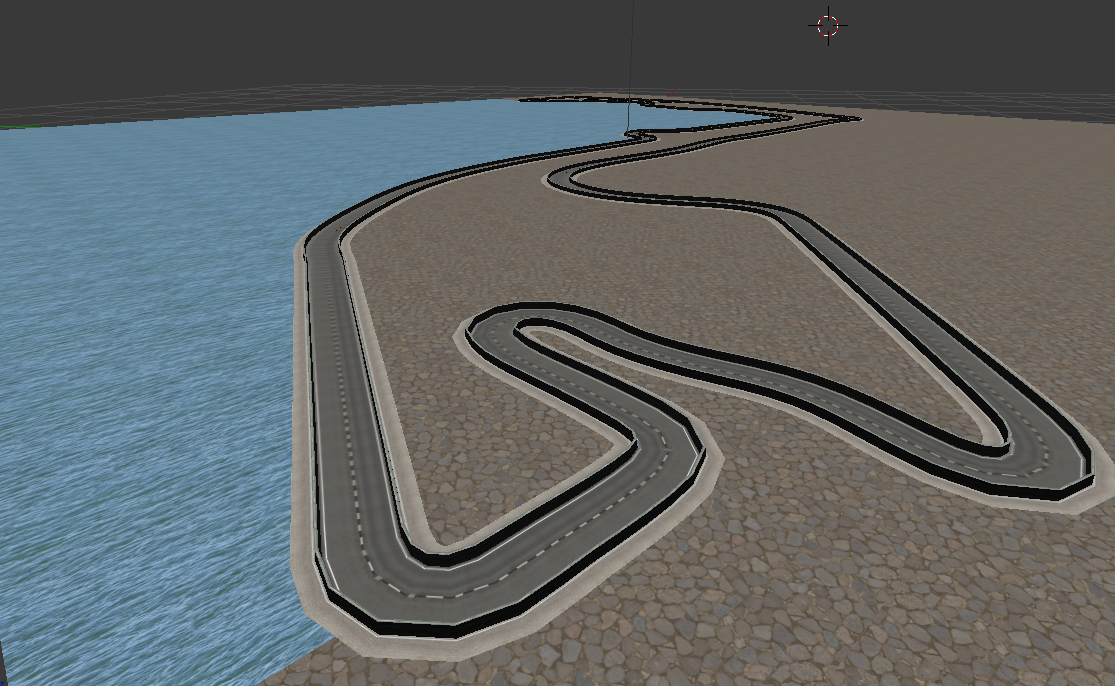
\includegraphics[width=0.47\textwidth]{MonacoPlano9.png}}\vspace{0.01\textwidth}
	\subfigure{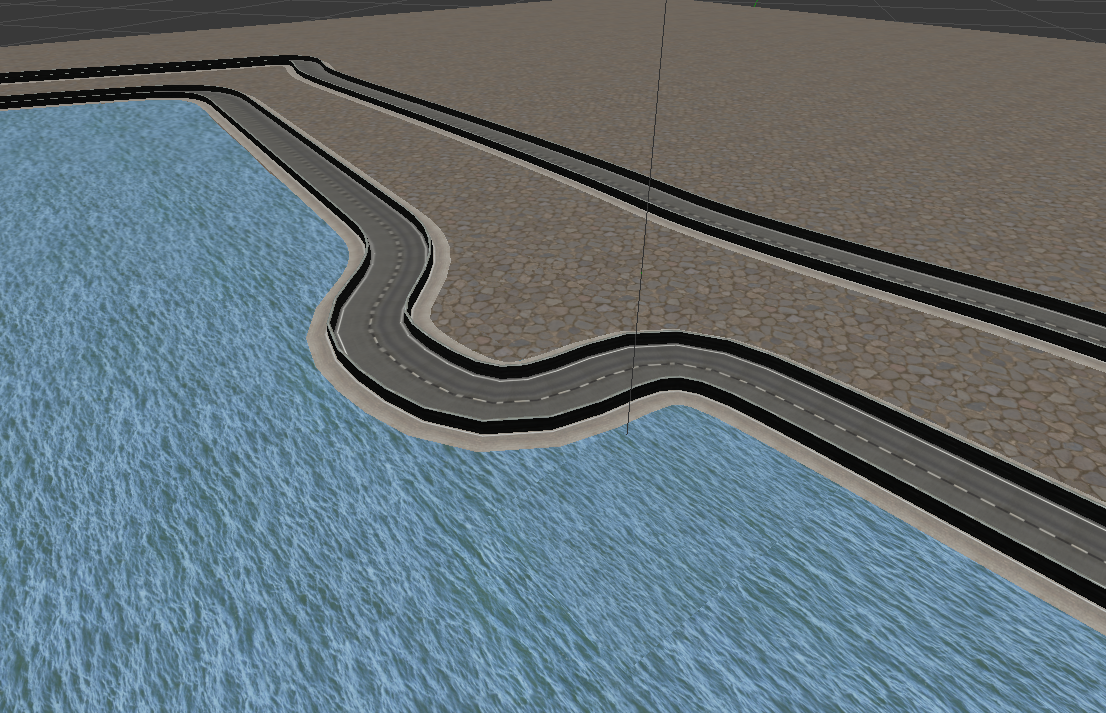
\includegraphics[width=0.47\textwidth]{MonacoPlano10.png}}\hspace{0.02\textwidth}
	\subfigure{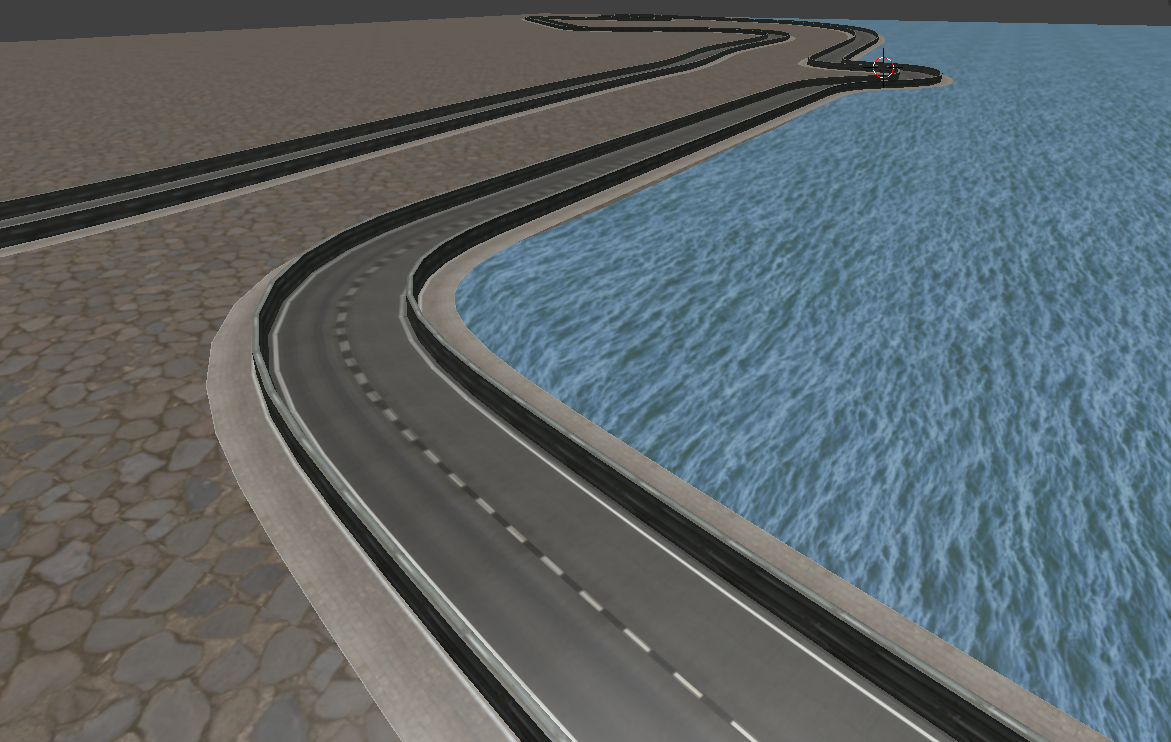
\includegraphics[width=0.47\textwidth]{MonacoPlano3.png}}
	\caption{Diferentes vistas del circuito de F1 de Mónaco plano.} \label{fig:monacoplanovistas}
\end{figure}


\section{Creación del circuito con elevaciones}
\label{sec:circarr_circuitoconelevaciones}

Una vez modelado el circuito plano pasamos a modelarlo ahora con elevaciones. Dada la dificultad de simplemente añadirlas al circuito ya creado, partimos de cero en la creación de este nuevo escenario. Puesto que ahora es mucho más relevante el fondo, comenzamos por esa parte. Eliminamos el cubo por defecto y añadimos un nuevo objeto, ésta vez una \textit{Mesh}, \textit{Grid}, que llamaremos rejilla. Es diferente del plano por que ya está subdividido, como una rejilla. Al crearlo, en la parte inferior izquierda de la ventana de vista 3D, aparecen una serie de propiedades únicas de este objeto que modificamos a nuestro gusto. En este caso el número de subdivisiones de la rejilla y el tamaño de ésta. Elegimos una cantidad moderada de divisiones ya que, aunque van a afectar visualmente a que las elevaciones no sean todo lo suaves que desearíamos, van a condicionar la carga de procesamiento del mundo en Gazebo, y queremos que sea todo lo ligera posible para poder realizar prácticas con múltiples objetos y vehículos sin que se vea comprometido el rendimiento.

Haciendo click en el botón de Modo Edición accedemos a otro modo, en este caso de Escultura. Una vez en este modo, en la parte superior izquierda de la ventana de vista 3D se despliega una multitud de herramientas y opciones para esculpir los objetos de la escena. Como lo que nos interesa es elevar la rejilla de forma que simule las alturas y elevaciones del circuito real de Mónaco, accedemos a la opción de bloqueo y seleccionamos los ejes x e y, con lo que sólo modificaremos la altura del plano sobre el que proyectaremos el trazado. Modificando las opciones del pincel hasta dejarlo a nuestro gusto comenzamos a esculpir la rejilla. Usando la misma imagen de antes como plantilla de fondo y fotos reales del circuito esculpimos un prototipo de lo que serán las elevaciones, que más tarde retocaremos para ajustarnos mejor a las peculiaridades del trazado. También nos serviremos de otro tipo de pincel para alisar las rugosidades creadas al modelar de forma más basta y así suavizar el terreno para acomodar mejor al circuito.

\begin{figure}[t]
	\centering
	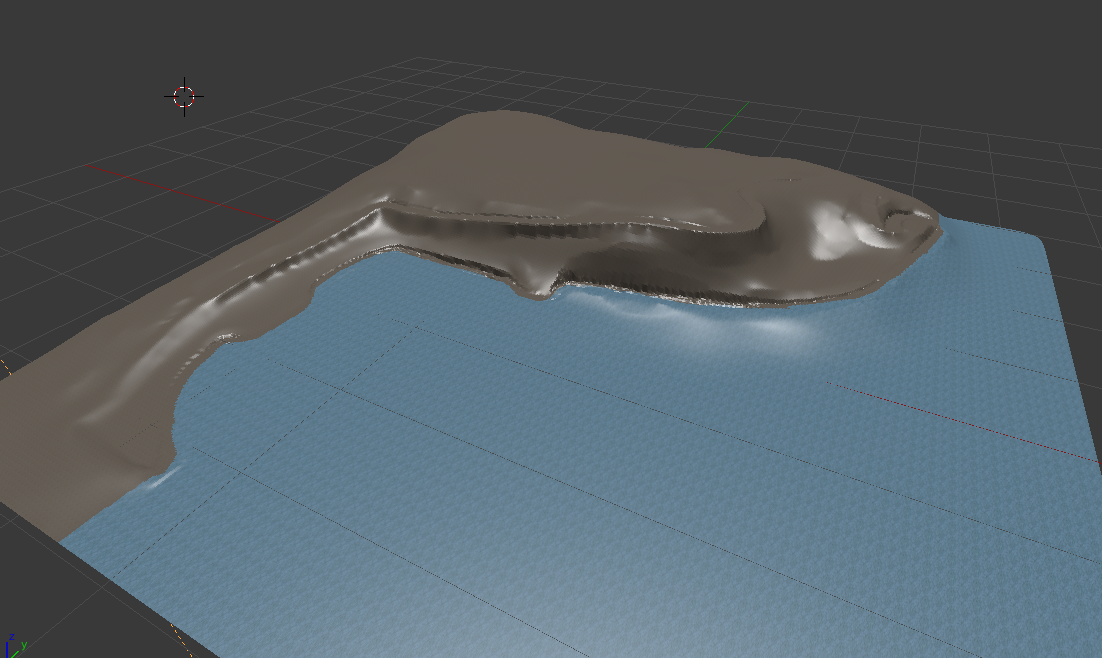
\includegraphics[width=0.75\textwidth]{MonacoElev00.png}
	\caption{Fondo para el circuito con elevaciones.} \label{fig:monacoelev00}
\end{figure}

A continuación creamos de nuevo, siguiendo los mismos pasos, la curva Bezier que servirá de trazado. Creamos ahora un plano, que pintamos de un color llamativo, y extendemos a lo largo de la curva bezier, consiguiendo un trazado de referencia para acabar de dar los últimos detalles a la rejilla. Tanto a la curva como a este plano le aplicamos como modificador la rejilla, consiguiendo darles altura y pudiendo ver el recorrido real del circuito con las elevaciones modeladas. Ahora modelamos la rejilla teniendo en cuenta el recorrido del circuito y su situación a orillas del mar, por lo que tenemos mucho cuidado de mantener plana toda la parte baja y del mar y aplicamos las elevaciones en las demás partes. Una vez modelado texturizamos de forma análoga a como hicimos anteriormente. Una vez modelado y texturizado el plano, eliminamos el trazado de referencia y obtenemos el suelo sobre el que descansará el circuito (\textit{Figura \ref{fig:monacoelev00}}).

Ahora repetiremos todos los pasos de creación del trazado (creamos el segmento, lo texturizamos, lo extendemos a lo largo de la curva) y además le aplicamos la rejilla como modificador. Si hemos realizado bien el paso anterior con el trazado de referencia, el trazado final debería descansar sobre la caja realizada y acoplarse perfectamente al terreno, de no ser así retocamos nuevamente la rejilla con las herramientas de escultura. 

\begin{figure}[hb]
	\centering
	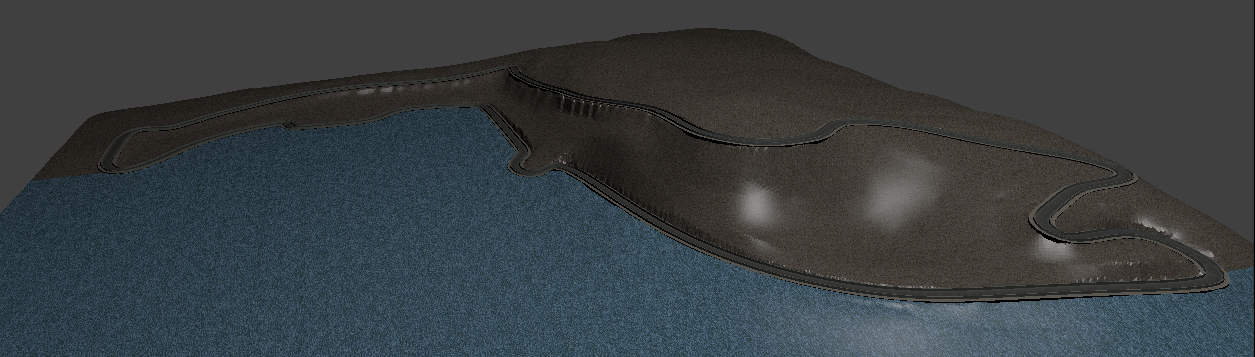
\includegraphics[width=1\textwidth]{MonacoElev05.png}
	\caption{Circuito con elevaciones.} \label{fig:monacoelev05}
\end{figure}

Una vez completado este paso podemos dar por finalizado el circuito (\textit{Figura \ref{fig:monacoelev05}}). En la Figura \ref{fig:monacoelevvistas} se pueden ver detalles del circuito donde se aprecian mejor las elevaciones del terreno.

\begin{figure}[h]
	\centering
	\subfigure{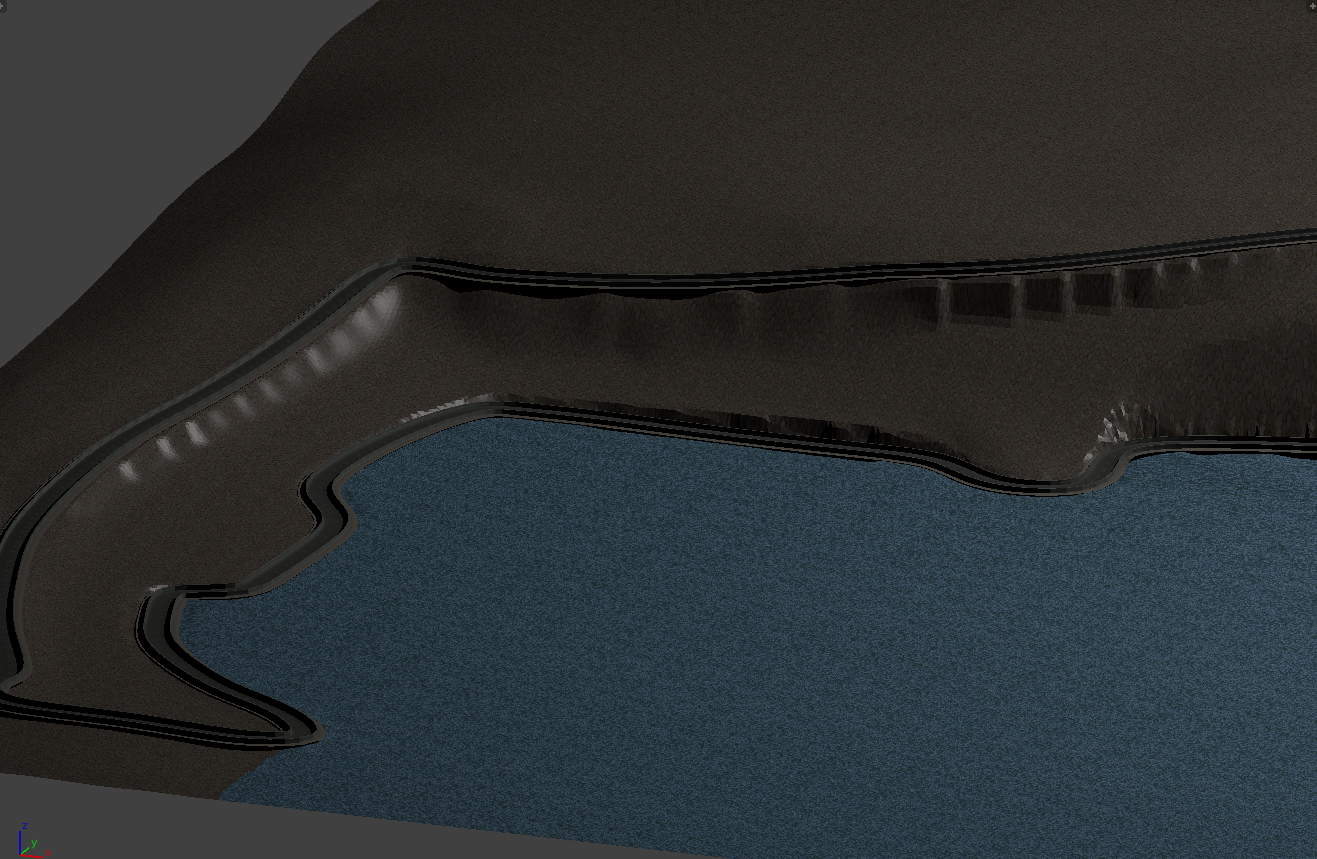
\includegraphics[width=0.495\textwidth]{MonacoElev01.png}}
	\subfigure{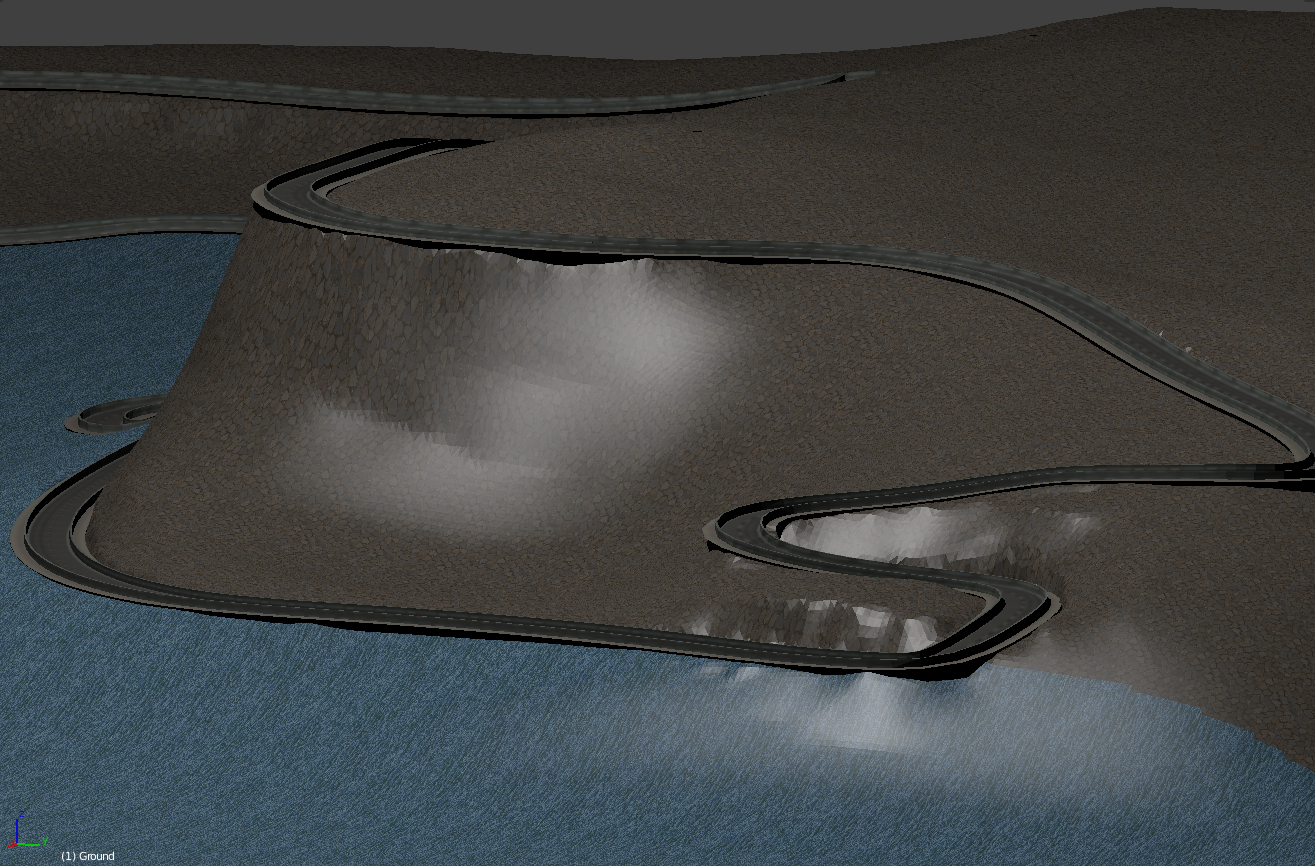
\includegraphics[width=0.495\textwidth]{MonacoElev02.png}}
	\subfigure{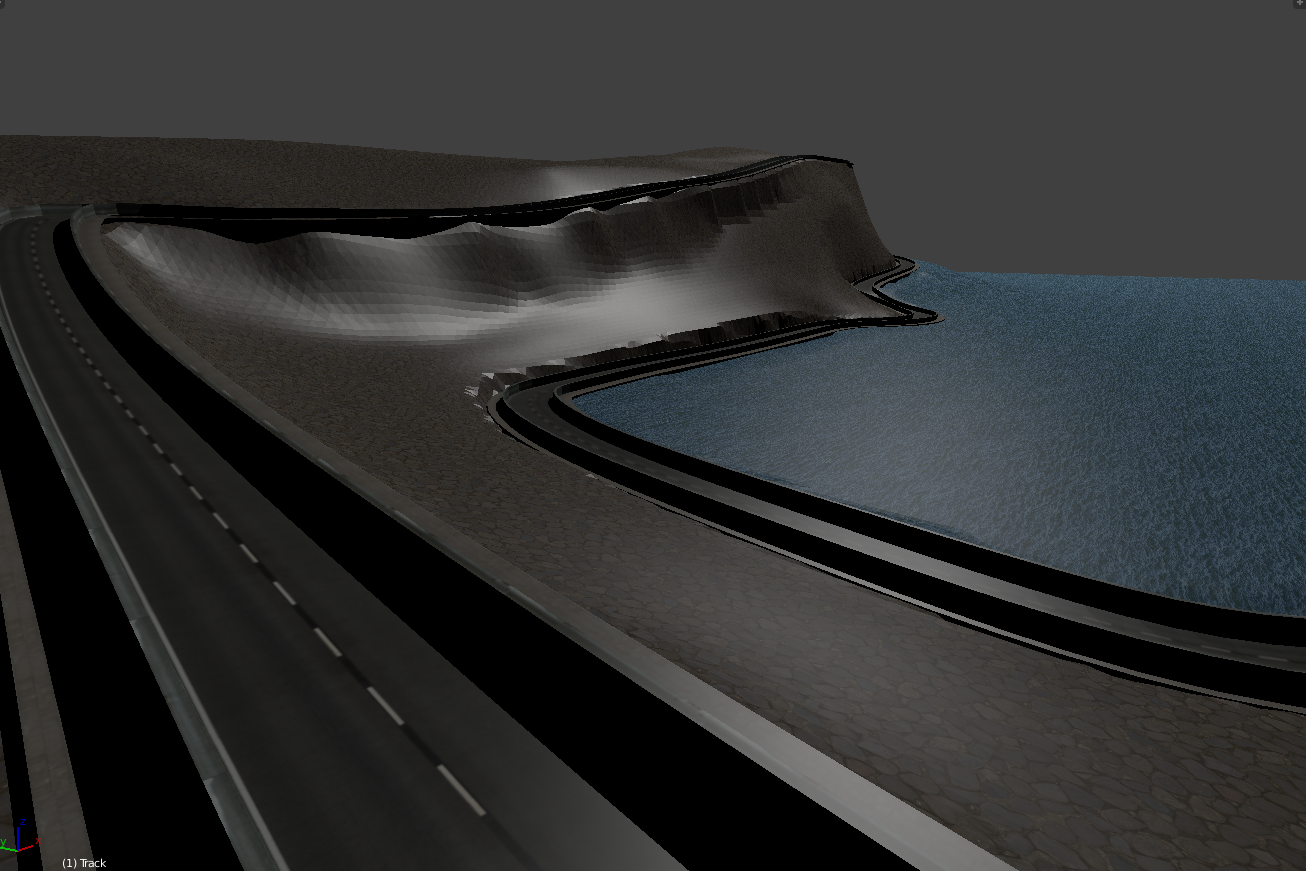
\includegraphics[width=0.495\textwidth]{MonacoElev03.png}}
	\subfigure{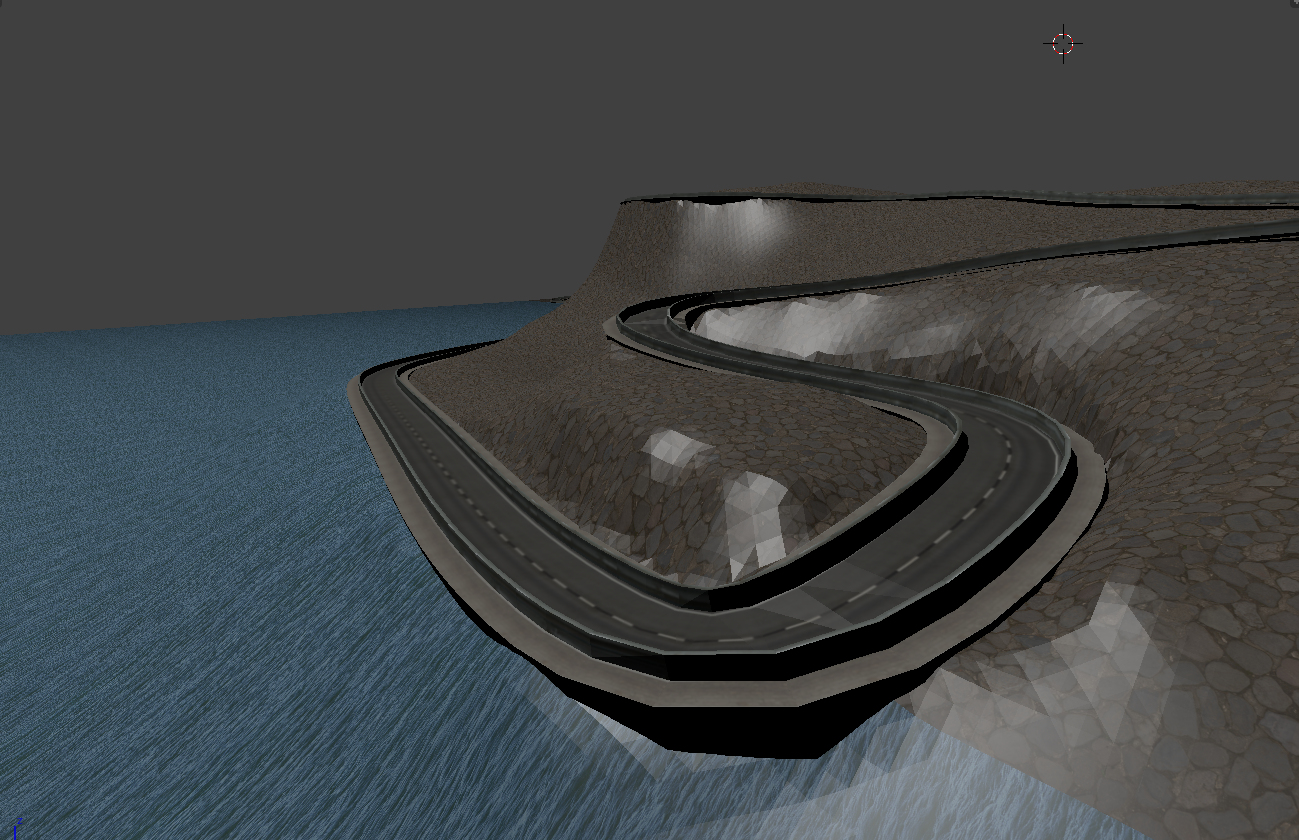
\includegraphics[width=0.495\textwidth]{MonacoElev04.png}}
	\caption{Diferentes vistas del circuito de F1 de Mónaco con elevaciones.} \label{fig:monacoelevvistas}
\end{figure}

Dado el carácter práctico de este escenario, y dado que ya existen prácticas desarrolladas con fines similares, procedemos a crear una variante del circuito, tanto el plano como el elevado, con una línea roja en el centro de su recorrido. Dicha línea servirá para realizar la práctica de control visual en la que es necesaria una referencia clara de un color determinado, siendo el rojo un color claramente diferente de cualquier componente del circuito como el asfalto o las vallas. Como podemos ver en la Figura \ref{fig:monacolinea} el circuito es idéntico en ambos casos salvo por la linea roja en el medio del asfalto. Para realizar esta modificación de la manera más eficiente y práctica realizamos unos pocos cambios al modelo original. Primero guardamos la escena con un nombre diferente para diferenciarlos. Después editamos la textura usada para crear el material del asfalto con un programa como GIMP\footnote{Siglas de “GNU Image Manipulation Program”, gratuito y de código abierto. \url{https://www.gimp.org/}} y le dibujamos esa línea roja. Después, en el nuevo fichero de Blender cambiamos, tanto en la textura como en el material asociado al asfalto, la imagen de fuente por la editada. Una vez hecho esto en ambos circuitos conseguimos esta variante más orientada a prácticas específicas. 

\begin{figure}[]
	\centering
	\subfigure[Mónaco plano.]{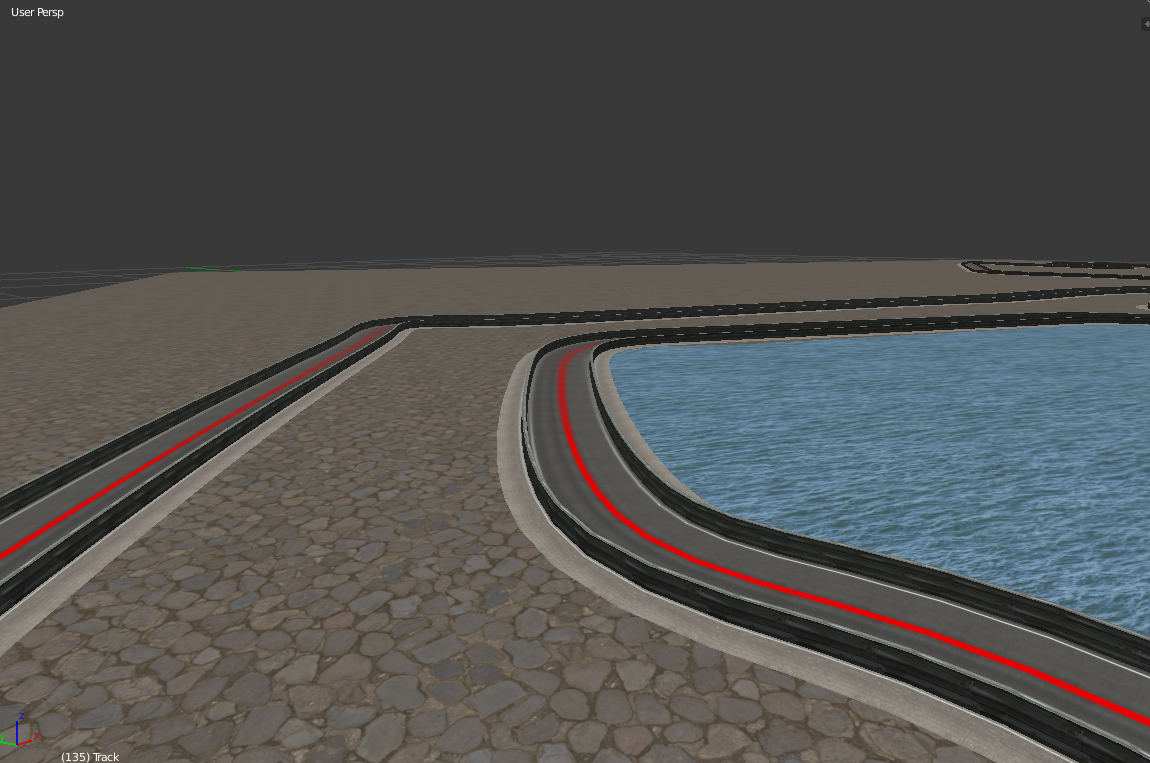
\includegraphics[width=0.49\textwidth]{monacolinea.png}}
	\subfigure[Mónaco con elevaciones.]{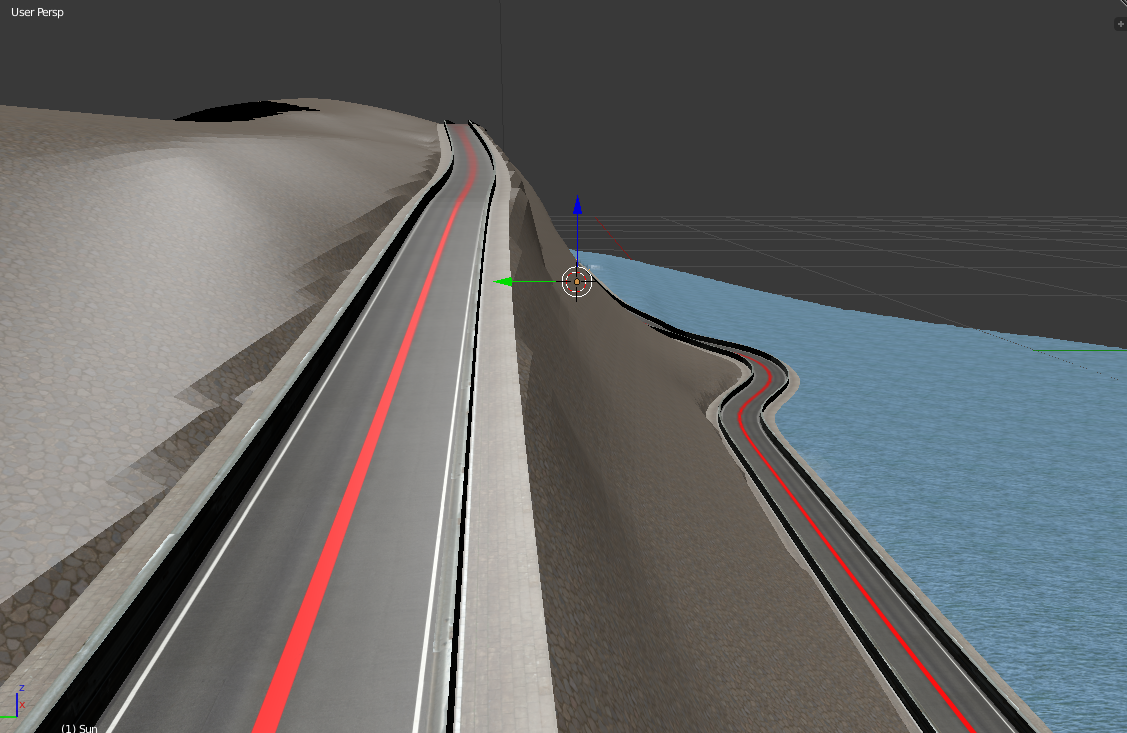
\includegraphics[width=0.5\textwidth]{monacoelevlinea.png}}
	\caption[Circuitos con una línea roja.]{Circuitos de mónaco editados para contener una línea roja en su trazado, tanto el plano (a) como el que contiene elevaciones (b).} \label{fig:monacolinea}
\end{figure}

\section{Mundos para Gazebo}
\label{sec:circarr_mundosparagazebo}

Ya hemos conseguido modelar dos escenarios, un circuito de Mónaco plano y otro con elevaciones, más realista. Pero aún no nos sirven, hemos de integrarlos en Gazebo para que puedan ser usados. Para ello estudiamos la estructura de los ficheros *.world de Gazebo, y vemos que se sirven de modelos en 3D en ficheros *.sdf y *.conf para componer los mundos. SDF\footnote{Página de SFD: \url{http://sdformat.org/}} es un formato XML que describe entornos y objetos para simuladores robóticos, visualización y control. Creado originalmente como parte de Gazebo, fué diseñado pensando en aplicaciones robóticas científicas, y ha evolucionado hasta convertirse en un formato robusto, estable y extensible capaz de describir objetos estáticos y dinámicos, terrenos, luces o físicas. 
Al analizar la estructura de los ficheros *.sdf observamos que importan los objetos que componen el mundo de otros ficheros en formatos como .mesh, .model, .dae, etc. Al comparar con otros mundo ya creados dentro de la plataforma JdeRobot vemos que muchos modelos están en formato .dae\footnote{Extensión asociada a los archivos Collada, esquema XML para transportar objetos 3D entre aplicaciones. \url{https://www.khronos.org/collada/}}. Así pues elegimos dicho formato para exportar el objeto desde Blender, comenzando primero con el circuito plano sin línea. Para ello hacemos click en el menú \textit{File}, \textit{Export}, \textit{Collada} (\textit{Figura \ref{fig:exportar}}).

\begin{figure}[h]
	\centering
	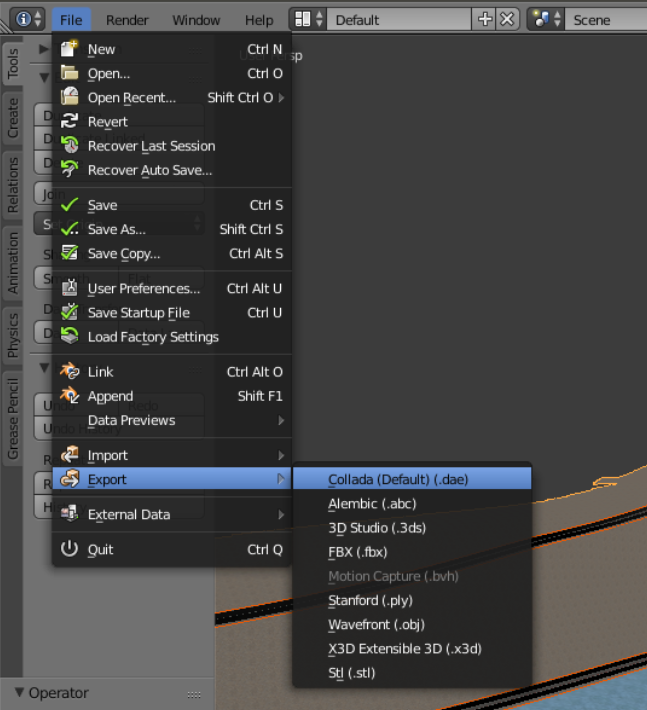
\includegraphics[width=0.6\textwidth]{exportar.png}
	\caption{Desplegable para exportar ficheros desde Blender.} \label{fig:exportar}
\end{figure}

En alguna versión de Blender esta opción no está disponible, por lo que hay que añadirla manualmente instalando desde fuente la extensión o buscar otra versión. En nuestro caso inicialmente instalamos la versión 2.76\textsubscript{b} y no tenía disponible esta opción. Optamos por instalar desde fuente la versión 2.78\textsubscript{c} que sí lo tiene. 

\begin{figure}[t]
	\centering
	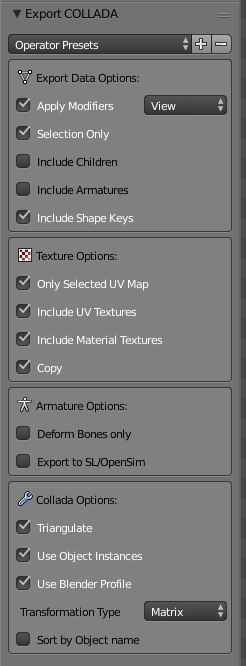
\includegraphics[width=0.3\textwidth]{exportcollada.png}
	\caption{Opciones de exportación de Collada.} \label{fig:exportcollada}
\end{figure}

Al seguir los pasos aparecemos en otra ventana de Blender donde nos pregunta la ruta donde exportar el archivo y el nombre del fichero, entre otros parámetros. Especialmente importantes son los que se aprecian en la Figura \ref{fig:exportcollada}. Si no se activan las casillas adecuadas se podrían producir errores en la exportación. Por ejemplo, dentro de \textit{Export Data Options} es necesario marcar tanto \textit{Apply Modifiers} como \textit{Selection Only}. La primera casilla sirve para no perder los modificadores aplicados a los objetos del escenario, como la curva o la rejilla aplicadas al segmento del circuito (\textit{Figura \ref{fig:monacosegmento}}). De no marcarlo podrían aparecer una fila de segmentos rectos y planos del circuito, o un circuito plano sobre las elevaciones, o un único segmento sin ninguno de los modificadores aplicados. 

El segundo es para exportar sólo los objetos seleccionados al hacer click en exportar. De esta manera podemos ayudarnos de múltiples objetos y mantenerlos en la escena para futuras modificaciones, o editar varios objetos a la vez en la misma escena pero exportarlos individualmente. De no marcar la casilla se exportarían todos los elementos de la escena. 

Dentro de \textit{Texture Options} se encuentran las opciones relaccionadas con las texturas. Aquí es necesario marcar las tres primeras casillas, \textit{Only Selected UV Map}, \textit{Include UV Textures}, \textit{Include Material Textures} y \textit{Copy}. Marcando la primera casilla se exportarán sólo las texturas de los objetos seleccionados, en lugar de todas las de la escena. La segunda y tercera casilla permiten exportar las texturas UV y los materiales usados respectivamente, de esta forma se mantienen las texturas que se veían en el modo de renderizado. Si simplemente asignamos una textura y no seguimos los pasos descritos anteriormente, en este paso Blender no las reconocería y no las exportaría junto con el resto del circuito, obteniendo así una figura sin imágenes en su superficie. 

La última casilla copia los archivos de las texturas a la carpeta de destino de la exportación, y los enlaza dentro del fichero .dae. De esta forma se pueden copiar los archivos resultantes a cualquier otro dispositivo sin perder ningún dato por el camino o hacer más configuración manual. Las secciones de \textit{Armature Options} y \textit{Collada Options} no son relevantes en nuestro caso, y con dejar las casillas marcadas por defecto es suficiente.

Una vez tenemos exportado el circuito a un fichero .dae, creamos el fichero .sdf que importaremos en el mundo de Gazebo. El fichero finalizado tendrá el siguiente contenido:

\lstset{language=xml}
\begin{lstlisting}
<?xml version='1.0'?>
<sdf version="1.4">
<model name="monaco">
	<static>true</static>
	<link name="monaco">
		<pose>0 0 0 0 0 0</pose>
		<collision name="collision">
			<geometry>
				<mesh>
					<scale>15 15 15</scale>
					<uri>model://monaco/meshes/CircuitoMonaco.dae</uri>
				</mesh>
			</geometry>
		</collision>
		<visual name="visual">
			<geometry>
				<mesh>
					<scale>15 15 15</scale>
					<uri>model://monaco/meshes/CircuitoMonaco.dae</uri>
				</mesh>
			</geometry>
		</visual>
	</link>
</model>
</sdf>
\end{lstlisting}

Dentro de este fichero podemos diferenciar claramente el campo \textit{link} entre las líneas 5 y 23. En este campo se importan los archivos y configuraciones que componen el modelo sdf. Podemos ver tres campos: \textit{pose}, \textit{collision} y \textit{visual}. El primero define la posición y la orientación del objeto. En nuestro caso, como estamos creando el modelo del mundo donde se situarán los demás objetos, podemos dejar cualquiera con tal de que esté minimamente centrado en el mundo. El segundo define las barreras de colisión con los demás objetos del mundo. Es importante dado que, de no incluirlo, Gazebo trataría el objeto como si de un holograma se tratase, permitiendo que cualquier otro objeto lo atravesase sin problemas. Y el tercero define la parte que se ve del objeto. Si no lo definimos obtendremos un circuito invisible. Ambos campos tienen definidos unos valores de \textit{scale}. Esto es así para mantener una cohesión con los demás mundos creados en JdeRobot y con los vehículos existentes. Es importante también el campo de la línea 4, \textit{static}, con valor \textit{true}. Este campo fuerza al circuito a quedarse inmóvil en el espacio de Gazebo y actuar como suelo para los coches. De no definirlo o no asignarle el valor \textit{true}, obtendremos un circuito que al comenzar la simulación de Gazebo caerá al vacío, junto con los demás objetos.

Para cumplir con el estándar de SDF es necesario también crear un fichero de configuración como este:
\lstset{language=xml}
\begin{lstlisting}
<?xml version="1.0"?>
	<model>
	<name>Monaco flat</name>
	<version>1.0</version>
	<sdf version='1.5'>model.sdf</sdf>

	<author>
		<name>Alvaro Villamil</name>
	</author>

	<description>
		The F1 Monaco track without elevations.
	</description>
</model>
\end{lstlisting}

De este fichero, de extensión .config, SDF extrae información como el nombre del modelo, la versión usada para crearlo, la descripción del mismo, el archivo al cual aplicar esta configuración o el autor.

A continuación estructuramos los ficheros para que mantengan coherencia con el resto de modelos de JdeRobot. De tal forma creamos una carpeta con el nombre del modelo, en este caso \textit{monaco}, y dentro de ella situamos los archivos \textit{model.config} y \textit{model.sdf} y una carpeta que llamamos \textit{meshes}. Dentro de esta carpeta guardamos el archivo \textit{CircuitoMonaco.dae} y todas las texturas que necesita nuestro modelo, tal y como las exportó Blender.

El siguiente paso es crear el fichero \textit{monaco.world}, el cual pasaremos como argumento a Gazebo al lanzarlo para que cargue nuestro mundo. Para decirle a Gazebo que queremos cargar nuestro circuito creamos el campo \textit{include} de las líneas 7 a 10. De esta manera le decimos que cargue el modelo \textit{monaco} y lo coloque en una posición en el mundo. También creamos un sol estándar de Gazebo en otro campo \textit{include}. Al probar a lanzar Gazebo con esta configuración vemos que la escena queda muy oscura y decidimos añadir dos \textit{light}, dos luces direccionales que además aportarán sombras y dinamismo al mundo. Para no crear una carga excesiva de trabajo de simulación hacemos que ambas luces sean idénticas, potenciando el efecto sin crear varias sombras ni reflejos innecesarios. El contenido final de dicho fichero es éste:
\\
\\
\\
\lstset{language=xml}
\begin{lstlisting}
<?xml version="1.0"?>
<sdf version="1.4">
	<world name="default">
		<include>
			<uri>model://sun</uri>
		</include>
		<include>
			<uri>model://monaco</uri>
			<pose>0 0 0 0 0 0</pose>
		</include>

		<light name='user_directional_light_0' type='directional'>
			<pose frame=''>0.467439 -3.3788 2.45574 0.487341 -0 0</pose>
			<diffuse>0.5 0.5 0.5 1</diffuse>
			<specular>0.1 0.1 0.1 1</specular>
			<direction>0.1 0.1 -0.9</direction>
			<attenuation>
				<range>20</range>
				<constant>0.5</constant>
				<linear>0.01</linear>
				<quadratic>0.001</quadratic>
			</attenuation>
			<cast_shadows>1</cast_shadows>
		</light>
		<light name='user_directional_light_1' type='directional'>
			<pose frame=''>0.467439 -3.3788 2.45574 0.487341 -0 0</pose>
			<diffuse>0.5 0.5 0.5 1</diffuse>
			<specular>0.1 0.1 0.1 1</specular>
			<direction>0.1 0.1 -0.9</direction>
			<attenuation>
				<range>20</range>
				<constant>0.5</constant>
				<linear>0.01</linear>
				<quadratic>0.001</quadratic>
			</attenuation>
			<cast_shadows>1</cast_shadows>
		</light>

	</world>
</sdf>
\end{lstlisting}

Para incorporarlo al conjunto de mundos y modelos de JdeRobot, primero comprobamos en nuestro ordenador que funciona correctamente. Para ello copiamos la carpeta \textit{monaco} con los archivos correspondientes al modelo dentro de la carpeta \textit{JdeRobot/src/drivers/gazeboserver/models}, y el fichero \textit{monaco.world} dentro de la carpeta \textit{JdeRobot/src/drivers/gazeboserver/worlds}. Al lanzar Gazebo con nuestro mundo como argumento no da ningún error y aparece el circuito correctamente. Una vez probado que todo funciona repetimos el proceso para cada circuito, obteniendo cuatro modelos y cuatro mundos, los correspondientes al circuito plano, al circuito con elevaciones, al circuito plano con la línea roja y al circuito con elevaciones con la línea roja. 

Sin embargo, las precauciones tomadas no han sido suficientes y los circuitos de Mónaco con elevaciones llevan una gran carga gráfica que hace que la simulación se mueva lenta. Para disminuir esta carga recortamos parte de la rejilla que sirve de fondo, reduciendo la zona del mar y la zona alta detrás del circuito. Son zonas lejanas al trazado que no van a disminuir la apariencia general, pero si a mejorar el rendimiento computacional. Una vez hecho este cambio comprobamos que la simulación en Gazebo se mueve con soltura y nos permite añadir objetos sin afectar al rendimiento. 

\begin{figure}[h]
	\centering
	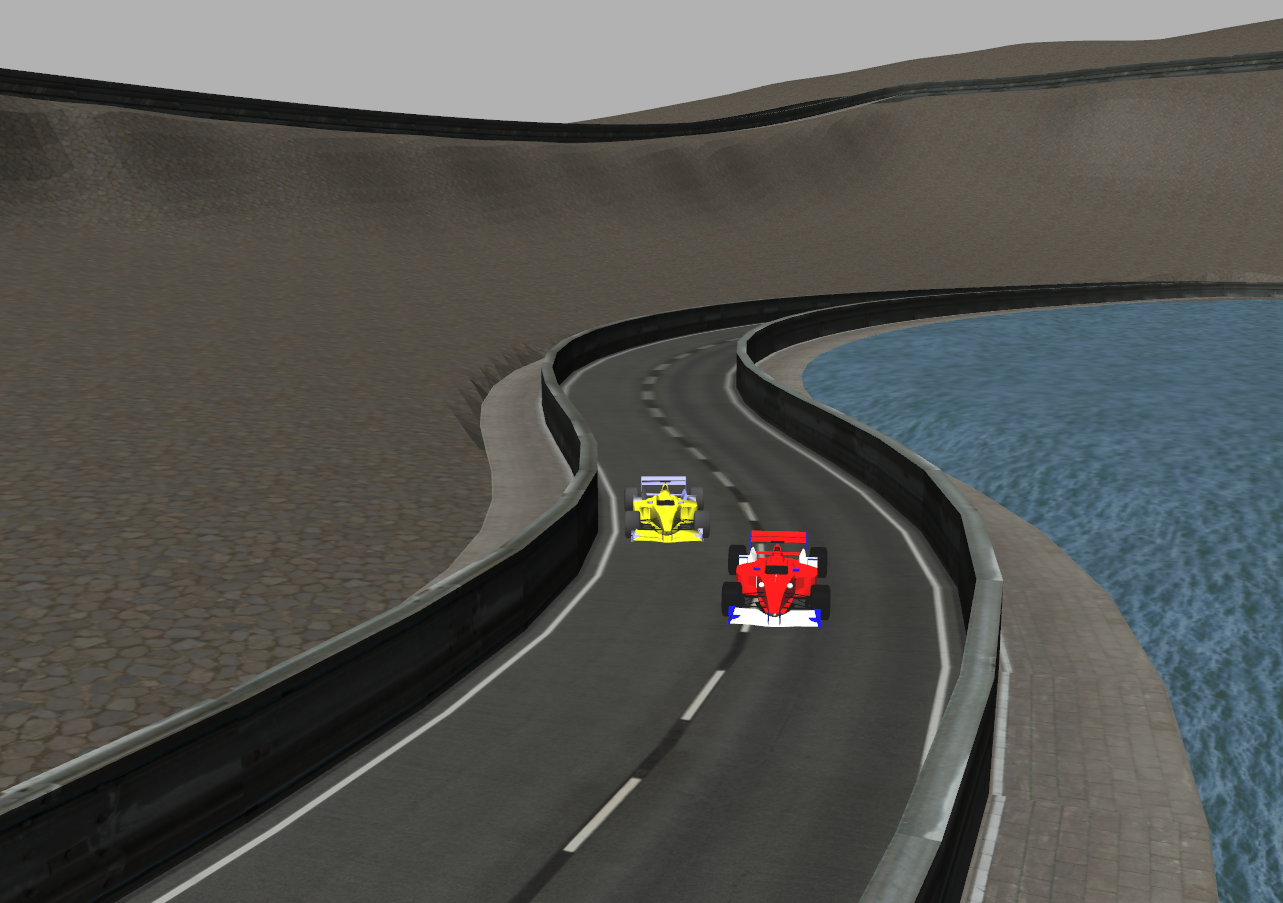
\includegraphics[width=0.75\textwidth]{MonacoElev08.png}
	\caption{Coches recorriendo el circuito de Mónaco.} \label{fig:monacocoches}
\end{figure}

Cuando ya hemos comprobado que con ninguno de los cuatro mundos se producen errores procedemos a hacer un \textit{pull} al repositorio oficial de JdeRobot\footnote{\url{https://github.com/JdeRobot/JdeRobot}} en GihHub. De esta forma logramos incorporar nuestros progresos al código oficial de JdeRobot, y que cualquiera que se descargue esta plataforma pueda disfrutar de los mundos que hemos creado. En la figura \ref{fig:monacocoches} podemos observar el resultado en Gazebo con coches circulando por el circuito como si de una práctica académica se tratase. También comprobamos que la fluidez del mundo al aumentar la carga de trabajo sigue siendo satisfactoria, y va a permitir realizar diferentes tipos de prácticas.

